\chapter{Comparative Analysis}
\thispagestyle{chapterstart}

In this chapter, we evaluate the feasibility and performance of various side-channel resistant implementations of the Dilithium signature scheme on embedded devices. We focus on how different countermeasures, specifically masking and shuffling techniques, affect security and efficiency. Through analysis of experimental results from existing studies, we assess the practicality of these implementations for real-world deployment.

\section{Vulnerability Assessment of Dilithium}

Understanding the susceptibility of Dilithium implementations to side-channel attacks is crucial for identifying necessary countermeasures. Table~\ref{tab:attack_surface} summarizes key findings from studies that evaluated the vulnerabilities of unprotected Dilithium implementations.

\begin{table}[ht]
    \centering
    \renewcommand{\arraystretch}{1.2}
    \caption{Attack Surface Assessment of Unprotected Dilithium Implementations}
    \label{tab:attack_surface}
    \begin{tabularx}{\textwidth}{|X|X|X|}
        \hline
        \textbf{Approach}                                             & \textbf{Evaluation Methodology}                        & \textbf{Findings}                                 \\ \hline
        Profiling attack on bit-unpacking function \cite{Marzougui22} & Machine learning profiling, integer linear programming & Full recovery of $s_1$ from 756,589 signatures    \\ \hline
        Side-channel attack on NTT \cite{Pessl19}                     & Single-trace analysis, factor graph modeling           & Secret key recovery from a single power trace     \\ \hline
        Leakage assessment \cite{Migliore19}                          & Welch's $t$-tests (500 traces), single-bit DPA         & Significant leakage detected with only 500 traces \\ \hline
    \end{tabularx}
\end{table}

Marzougui et al.~\cite{Marzougui22} demonstrated that the bit-unpacking function in Dilithium leaks sensitive information. Using machine learning and integer linear programming on power traces from 756,589 signatures, they fully recovered the secret key component $s_1$, highlighting a severe vulnerability in unprotected implementations.

Pessl et al.~\cite{Pessl19} exploited deterministic patterns in the NTT computations to recover secret keys from a single power trace. By applying factor graph modeling and belief propagation, they showed that the NTT is a significant source of side-channel leakage.

Migliore et al.~\cite{Migliore19} conducted leakage assessments using Welch's $t$-tests and single-bit \ac{DPA} on unprotected implementations. They observed significant leakage with as few as 500 traces, confirming that sensitive information can be extracted without sophisticated attacks.

These studies collectively demonstrate that unprotected Dilithium implementations are highly susceptible to side-channel attacks, necessitating effective countermeasures to ensure security on embedded devices.

\section{Evaluation of Side-Channel Countermeasures}

Various countermeasures have been proposed to mitigate side-channel vulnerabilities in Dilithium. Table~\ref{tab:countermeasures} summarizes these methods, their evaluation approaches, security frameworks, and key findings regarding their effectiveness.

\begin{table}[ht]
    \centering
    \renewcommand{\arraystretch}{1.2}
    \caption{Evaluation of Side-Channel Countermeasures for Dilithium}
    \label{tab:countermeasures}
    \begin{tabularx}{\textwidth}{|X|X|X|X|}
        \hline
        \textbf{Countermeasure}                 & \textbf{Evaluation Methodology}                & \textbf{Security Framework}           & \textbf{Findings}                 \\ \hline
        High-order masking \cite{Migliore19}    & Statistical tests on 10,000 traces             & $t$-probing security                  & No detectable leakage observed    \\ \hline
        Randomized masking \cite{Azouaoui22}    & Sensitivity analysis, bitsliced implementation & Improved sensitivity analysis         & Enhanced leakage protection;      \\ \hline
        Improved masking gadgets \cite{Coron23} & Simulations, formal proofs,                    & $t$-probing, $t$-NI, $t$-SNI security & Secure gadgets; higher overheads; \\ \hline
        Shuffling techniques \cite{Ravi20}      & Practical evaluation on ARM Cortex-M4          & Randomization entropy metrics         & Reduced traceability;             \\ \hline
    \end{tabularx}
\end{table}

Migliore et al.~\cite{Migliore19} implemented high-order masking techniques and evaluated their effectiveness using statistical analysis on 10,000 traces. Their results showed no detectable leakage, confirming the robustness of their countermeasures under the $t$-probing security model.

Azouaoui et al.~\cite{Azouaoui22} refined sensitivity analysis to identify critical operations requiring protection and introduced randomized masking schemes with bitsliced implementations. This approach enhanced leakage protection while improving performance, particularly at higher masking orders.

Coron et al.~\cite{Coron23} developed new masking gadgets, such as the ShiftMod gadget, and validated their security through simulations and formal proofs. Although their implementation incurred higher overheads, it serves as a proof-of-concept, demonstrating strong security under the $t$-SNI model. They suggest that performance can be improved through architecture-specific optimizations and bitslicing.

Ravi et al.~\cite{Ravi20} explored shuffling techniques on an ARM Cortex-M4 microcontroller. Their evaluations indicated that shuffling reduces traceability, with the level of security improvement varying based on the shuffling method employed.

\section{Performance Impact of Countermeasures}

Implementing side-channel countermeasures affects the performance of Dilithium operations, particularly key generation and signing. We analyze the execution time overhead introduced by different countermeasures, using the unprotected implementation as a baseline (normalized execution time of 1)\footnote{Normalized execution time is the ratio of the protected implementation's execution time to the unprotected implementation's, measuring the overhead of side-channel countermeasures.}.

\subsubsection{Key Generation Performance}

Figure~\ref{fig:keygen_performance} compares the normalized execution times for key generation with various countermeasures.

\begin{figure}[ht]
    \centering
    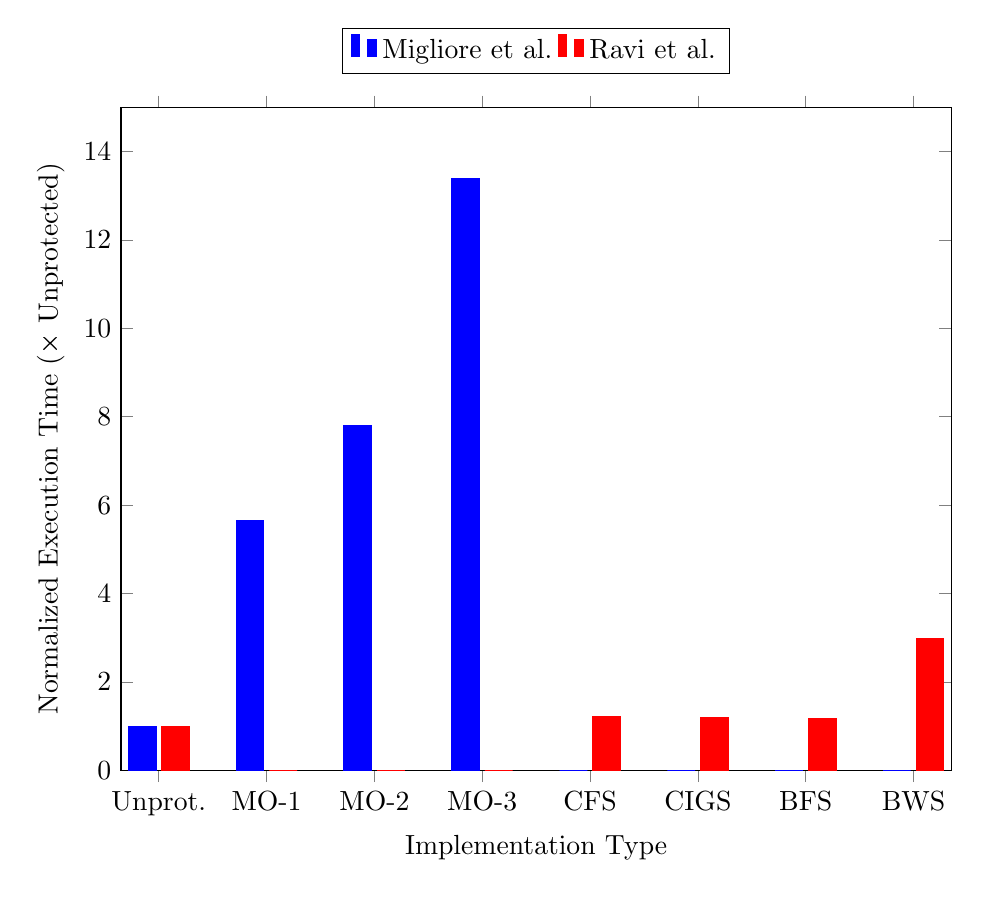
\begin{tikzpicture}
        \begin{axis}[
                ybar,
                bar width=10pt,
                width=\textwidth,
                height=10cm,
                legend style={at={(0.5,1.05)},
                        anchor=south,legend columns=-1},
                symbolic x coords={
                        Unprot.,
                        MO-1,
                        MO-2,
                        MO-3,
                        CFS,
                        CIGS,
                        BFS,
                        BWS
                    },
                xtick=data,
                ylabel={Normalized Execution Time (× Unprotected)},
                xlabel={Implementation Type},
                ymin=0,
                ymax=15,
                enlarge x limits=0.05,
                x tick label style={font=\normalsize},
                y tick label style={/pgf/number format/fixed},
            ]
            \addplot[blue,fill=blue] coordinates {
                    (Unprot.,1)
                    (MO-1,5.66)
                    (MO-2,7.8)
                    (MO-3,13.4)
                    (CFS,0)
                    (CIGS,0)
                    (BFS,0)
                    (BWS,0)
                };

            \addplot[red,fill=red] coordinates {
                    (Unprot.,1)
                    (MO-1,0)
                    (MO-2,0)
                    (MO-3,0)
                    (CFS,1.221)
                    (CIGS,1.203)
                    (BFS,1.181)
                    (BWS,2.971)
                };

            \legend{Migliore et al., Ravi et al.}
        \end{axis}
    \end{tikzpicture}
    \caption{Normalized execution time of Dilithium KeyGen for different implementations.}
    \label{fig:keygen_performance}
\end{figure}

High-order masking, as implemented by Migliore et al.~\cite{Migliore19}, significantly increases execution time due to the overhead of securely processing multiple shares. For instance, masking order 1 (MO-1) increases execution time by approximately 5.66 times, while masking order 3 (MO-3) increases it to 13.4 times.

In contrast, shuffling techniques evaluated by Ravi et al.~\cite{Ravi20} introduce moderate performance overheads. Coarse shuffling methods, such as Coarse-Full Shuffle (CFS) and Coarse In-Group Shuffle (CIGS), increase execution time by about 1.2 times. Bitwise Fine Shuffling (BWS) incurs a higher overhead of approximately 2.97 times due to its increased computational complexity.

\subsubsection{Signing Performance}

Figure~\ref{fig:combined_performance_updated} illustrates the normalized execution times for the signing operation with different countermeasures.

\begin{figure}[ht]
    \centering
    \begin{subfigure}[b]{0.45\textwidth}
        \centering
        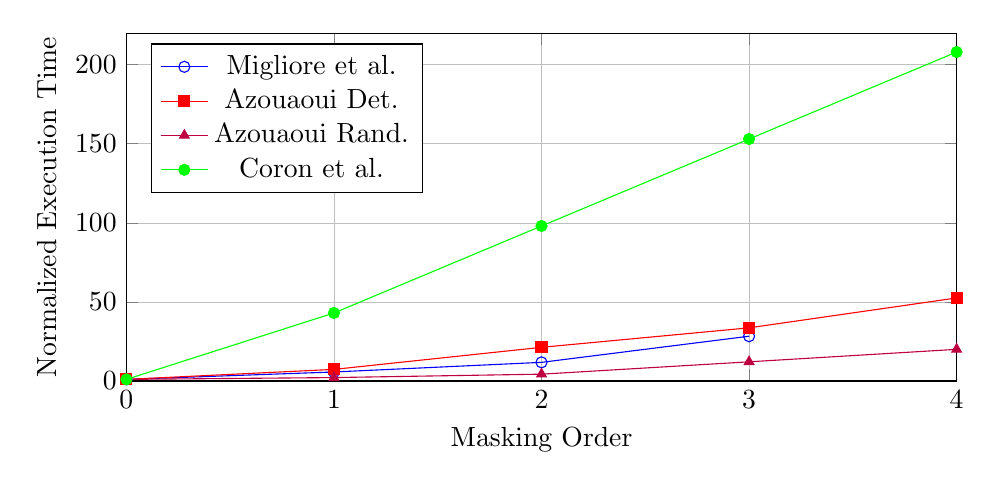
\begin{tikzpicture}
            \begin{axis}[
                    width=\textwidth,
                    height=6cm,
                    xlabel={Masking Order},
                    ylabel={Normalized Execution Time},
                    xmin=0, xmax=4,
                    ymin=0, ymax=220,
                    xtick={0,1,2,3,4},
                    ytick={0,50,100,150,200},
                    legend pos=north west,
                    grid=both,
                    grid style={line width=.1pt, draw=gray!10},
                    major grid style={line width=.2pt,draw=gray!50},
                ]
                % Migliore data
                \addplot[color=blue,mark=o] coordinates {
                        (0,1)
                        (1,5.68)
                        (2,11.77)
                        (3,28.3)
                    };
                \addlegendentry{Migliore et al.}

                % Azouaoui Deterministic data
                \addplot[color=red,mark=square*] coordinates {
                        (0,1)
                        (1,7.32)
                        (2,21.27)
                        (3,33.6)
                        (4,52.5)
                    };
                \addlegendentry{Azouaoui Det.}

                % Azouaoui Randomized data
                \addplot[color=purple,mark=triangle*] coordinates {
                        (0,1)
                        (1,2.15)
                        (2,4.3)
                        (3,12.11)
                        (4,20)
                    };
                \addlegendentry{Azouaoui Rand.}

                % Coron data
                \addplot[color=green,mark=*] coordinates {
                        (0,1)
                        (1,43)
                        (2,98)
                        (3,153)
                        (4,208)
                    };
                \addlegendentry{Coron et al.}

            \end{axis}
        \end{tikzpicture}
        \caption{Masking Implementations}
        \label{fig:masking_performance_line}
    \end{subfigure}
    \hfill
    \begin{subfigure}[b]{0.45\textwidth}
        \centering
        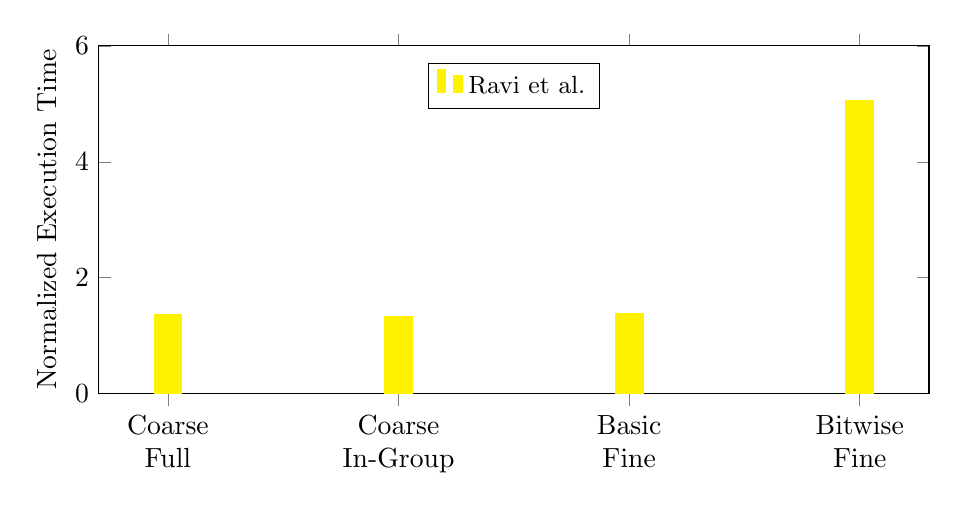
\begin{tikzpicture}
            \begin{axis}[
                    ybar=0pt,
                    bar width=10pt,
                    width=\textwidth,
                    height=6cm,
                    legend style={
                            at={(0.5,0.95)},
                            anchor=north,
                            draw=black,
                            font=\small
                        },
                    symbolic x coords={
                            {Coarse\\Full},
                            {Coarse\\In-Group},
                            {Basic\\Fine},
                            {Bitwise\\Fine}
                        },
                    xtick=data,
                    ylabel={Normalized Execution Time},
                    ymin=0,
                    ymax=6,
                    enlarge x limits=0.10,
                    x tick label style={font=\normalsize, align=center},
                    y tick label style={/pgf/number format/fixed},
                ]
                \addplot[yellow,fill=yellow] coordinates {
                        ({Coarse\\Full},1.359)
                        ({Coarse\\In-Group},1.338)
                        ({Basic\\Fine},1.377)
                        ({Bitwise\\Fine},5.06)
                    };

                \legend{Ravi et al.}
            \end{axis}
        \end{tikzpicture}
        \caption{Shuffling Implementations}
        \label{fig:shuffle_performance}
    \end{subfigure}
    \caption{Normalized execution time of Dilithium Signing for masking and shuffling implementations.}
    \label{fig:combined_performance_updated}
\end{figure}

Migliore et al.~\cite{Migliore19} observed that higher masking orders substantially increase signing execution time. MO-1 incurs approximately 5.68 times the execution time of the unprotected version, while MO-3 reaches 28.3 times.

Azouaoui et al.~\cite{Azouaoui22} achieved better performance with their randomized masking scheme, reducing the overhead at higher masking orders. For example, MO-2 incurs approximately 4.3 times the execution time of the unprotected implementation, benefiting from efficient randomness handling and optimized masking gadgets.

Coron et al.~\cite{Coron23} reported higher overheads, particularly at higher masking orders, with execution times increasing up to 208 times the unprotected version at MO-4. However, their implementation was a non-optimized proof-of-concept, and they anticipate significant performance improvements through optimizations.

Shuffling techniques generally incur lower performance overheads compared to masking. Ravi et al.~\cite{Ravi20} found that shuffling methods increased signing execution time by factors ranging from 1.18 to 5.06, depending on the granularity of shuffling.

\section{Discussion}

The comparative analysis reveals a trade-off between security and performance when implementing side-channel countermeasures in Dilithium. High-order masking provides strong security guarantees under rigorous models like the $t$-probing model but introduces significant performance overheads. This may not be practical for resource-constrained embedded devices without optimization.

Optimized implementations, such as those by Azouaoui et al.~\cite{Azouaoui22}, demonstrate that performance penalties can be mitigated through careful design, bitslicing, and hardware-specific optimizations. By targeting critical operations and employing efficient masking gadgets, they achieved better performance at higher masking orders.

Shuffling techniques offer a balance between security and performance. While they generally provide less robust security compared to high-order masking, they introduce lower overheads and can be effective against certain types of attacks, especially when combined with other countermeasures.

Practitioners must consider specific security requirements, performance constraints, and hardware characteristics when selecting countermeasures. The choice between masking and shuffling, or a combination thereof, depends on the desired level of security and acceptable performance impact.

Future research could explore hybrid approaches that integrate masking with shuffling or bitslicing to enhance both security and efficiency. Additionally, optimizing implementations for specific architectures and mitigating micro-architectural leakages remain important areas for development.
